\documentclass[border=15pt]{standalone}
\usepackage{tikz}
\usetikzlibrary{arrows.meta, positioning, calc}
\usepackage{amsmath}

\begin{document}

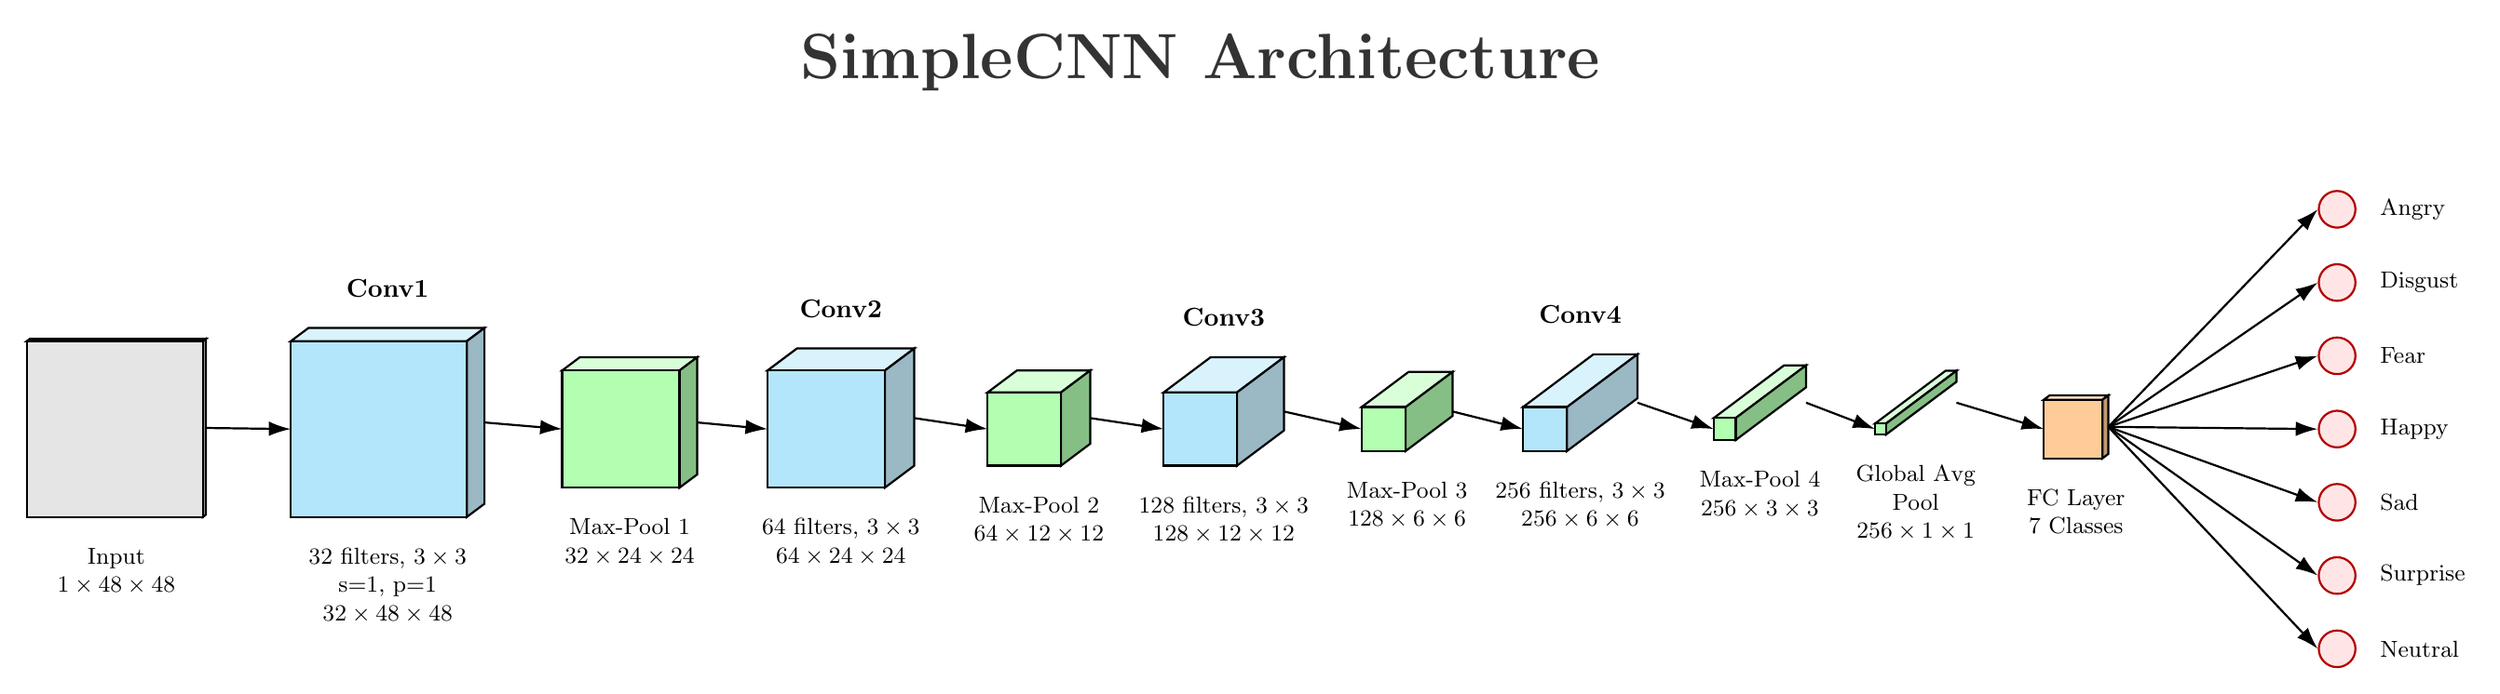
\begin{tikzpicture}[
    x=1cm, y=1cm,
    font=\sffamily,
    >= {Latex[length=3mm, width=2mm]},
    ]

    % Define a macro to draw each 3D layer block
    \newcommand{\networklayer}[7]{
        \def\posx{#2}
        \def\spat{#3}
        \def\chan{#4}

        % Perspective projection adjustments
        \pgfmathsetmacro{\cx}{\chan * 0.4}
        \pgfmathsetmacro{\cy}{\chan * 0.3}

        % 【修复颜色解析报错】
        % 先将带百分号的输入颜色（如 cyan!30）存为一个干净的中间变量 basecolor
        \colorlet{basecolor}{#5}
        % 然后基于中间变量进行亮度调节
        \colorlet{frontcolor}{basecolor}
        \colorlet{topcolor}{basecolor!50!white}
        \colorlet{sidecolor}{basecolor!75!black}

        % Draw Top Face
        \draw[fill=topcolor, thick] (\posx, \spat/2) -- (\posx + \spat, \spat/2) -- (\posx + \spat + \cx, \spat/2 + \cy) -- (\posx + \cx, \spat/2 + \cy) -- cycle;
        % Draw Right Face
        \draw[fill=sidecolor, thick] (\posx + \spat, -\spat/2) -- (\posx + \spat + \cx, -\spat/2 + \cy) -- (\posx + \spat + \cx, \spat/2 + \cy) -- (\posx + \spat, \spat/2) -- cycle;
        % Draw Front Face
        \draw[fill=frontcolor, thick] (\posx, -\spat/2) rectangle (\posx + \spat, \spat/2);

        % Define Anchor Coordinates for arrows
        \coordinate (in-#1) at (\posx, 0);
        \coordinate (out-#1) at (\posx + \spat + \cx, \cy/2);
        
        % Label Nodes
        \node[align=center, anchor=south, yshift=0.3cm, font=\bfseries] at (\posx + \spat/2 + \cx/2, \spat/2 + \cy) {#6};
        \node[align=center, anchor=north, yshift=-0.3cm, font=\small] at (\posx + \spat/2 + \cx/2, -\spat/2) {#7};
    }

    % ==========================================
    % Draw Network Layers
    % ==========================================
    \networklayer{input}{0}{2.4}{0.1}{gray!20}{}{Input \\ $1 \times 48 \times 48$}
    \networklayer{conv1}{3.6}{2.4}{0.6}{cyan!30}{Conv1}{32 filters, $3 \times 3$ \\ s=1, p=1 \\ $32 \times 48 \times 48$}
    \networklayer{pool1}{7.3}{1.6}{0.6}{green!30}{}{Max-Pool 1 \\ $32 \times 24 \times 24$}
    \networklayer{conv2}{10.1}{1.6}{1.0}{cyan!30}{Conv2}{64 filters, $3 \times 3$ \\ $64 \times 24 \times 24$}
    \networklayer{pool2}{13.1}{1.0}{1.0}{green!30}{}{Max-Pool 2 \\ $64 \times 12 \times 12$}
    \networklayer{conv3}{15.5}{1.0}{1.6}{cyan!30}{Conv3}{128 filters, $3 \times 3$ \\ $128 \times 12 \times 12$}
    \networklayer{pool3}{18.2}{0.6}{1.6}{green!30}{}{Max-Pool 3 \\ $128 \times 6 \times 6$}
    \networklayer{conv4}{20.4}{0.6}{2.4}{cyan!30}{Conv4}{256 filters, $3 \times 3$ \\ $256 \times 6 \times 6$}
    \networklayer{pool4}{23.0}{0.3}{2.4}{green!30}{}{Max-Pool 4 \\ $256 \times 3 \times 3$}
    \networklayer{gap}{25.2}{0.15}{2.4}{green!30}{}{Global Avg \\ Pool \\ $256 \times 1 \times 1$}
    \networklayer{fc}{27.5}{0.8}{0.2}{orange!40}{}{FC Layer \\ 7 Classes}

    % ==========================================
    % Draw Arrows Between Layers
    % ==========================================
    \draw[->, thick] (out-input) -- (in-conv1);
    \draw[->, thick] (out-conv1) -- (in-pool1);
    \draw[->, thick] (out-pool1) -- (in-conv2);
    \draw[->, thick] (out-conv2) -- (in-pool2);
    \draw[->, thick] (out-pool2) -- (in-conv3);
    \draw[->, thick] (out-conv3) -- (in-pool3);
    \draw[->, thick] (out-pool3) -- (in-conv4);
    \draw[->, thick] (out-conv4) -- (in-pool4);
    \draw[->, thick] (out-pool4) -- (in-gap);
    \draw[->, thick] (out-gap) -- (in-fc);

    % ==========================================
    % Draw Output Nodes
    % ==========================================
    \coordinate (node_start) at (31.5, 0);

    \foreach \name/\y/\label in {
        angry/3/Angry, 
        disgust/2/Disgust, 
        fear/1/Fear, 
        happy/0/Happy, 
        sad/-1/Sad, 
        surprise/-2/Surprise, 
        neutral/-3/Neutral} 
    {
        \node[circle, draw=red!70!black, fill=red!10, thick, minimum size=0.5cm] (outnode-\name) at (31.5, \y) {};
        \node[right=0.2cm of outnode-\name, font=\small] {\label};
        \draw[->, thick] (out-fc) -- (outnode-\name.west);
    }

    % ==========================================
    % Title
    % ==========================================
    \node[font=\Huge\bfseries, align=center, text=black!80] at (16, 5) {SimpleCNN Architecture};

\end{tikzpicture}

\end{document}
